\chapter{Second Order Boundary Value Problems}

\section{2nd order two-point boundary value problems}

\begin{intro}
  We have already seen, that boundary value problems have very
  different stability properties than initial value
  problems. Here, we will discuss a special class of boundary value
  problems of the form
  \begin{gather}
    \label{eq:bvp-second:1}
    -u''(x) + \beta(x) u'(x) + \gamma(x)u(x) = f(x),
    \qquad u(a) = u_a,
    \quad u(b) = u_b.
  \end{gather}

  In order to make this problem more amenable to mathematical
  investigation, we introduce the set
  \begin{gather*}
    \mathcal B =
    \Bigl\{ u\in C^2(a,b) \cap C[a,b]
    \;\Big|\; u(a) = u_a\;\wedge\; u(b) = u_b
    \Bigr\}.
  \end{gather*}

  Then, we can see the left hand side of the differential equation as
  a differential operator applied to $u$ and thus mapping $\mathcal B$
  to the set of continuous functions. Namely, we define
  \begin{gather}
    \label{eq:fd:2}
    \begin{split}
      L: \mathcal B &\to C[a,b] \\
      u & \mapsto -u'' + \beta u' + \gamma u.
    \end{split}
  \end{gather}
  In addition, we would like to simplify our life and get rid of the
  inhomogeneous boundary values $u_a$ and $u_b$. To this end, let
  \begin{gather*}
    u_B(x) = u_a \frac{b-x}{b-a} + u_b \frac{x-a}{b-a},
  \end{gather*}
  and introduce the new function $u_0 = u+u_B$. Then, $u_0$ solves
  the boudnary value problem
  \begin{multline*}
    -u_0''(x) + \beta(x) u'(x) + \gamma(x)u(x) = f(x) -
    \beta(x)\frac{u_b-u_a}{b-a} - \gamma(x)u_B(x),
    \\ u(a) =  u(b) = 0.
  \end{multline*}
  Thus, it is sufficient to consider the boundary value problem
\end{intro}

\begin{Definition}{bvp-second}
  Given an interval $I=[a,b]$, find a function
  \begin{gather}
    \label{eq:bvp-second:3}
    u\in V = \Bigl\{u\in C^2(a,b) \cap C[a,b]
	\;\Big|\; u(a) = u(b) = 0 \Bigr\},
  \end{gather}
  such that for a differential operator of second order as defined
  above and a right hand side $f\in C[a,b]$ there holds
  \begin{gather}
    \label{eq:bvp-second:2}
    Lu = f.
  \end{gather}
\end{Definition}
%%% Local Variables:
%%% mode: latex
%%% TeX-master: "../notes"
%%% End:


\begin{remark}
  This definition exhibits a major change in paradigm. Before, we
  considered a differential equation as an equation which determines
  the derivative of a function in a point. Now, we are looking at a
  linear system of equations, albeit one, which is not of finite
  dimension. This paradigm change will be essential when we consider
  partial differential equations in future semesters.
  
  On the other hand, the equality in equation~\eqref{eq:bvp-second:2}
  is understood point-wise, such that in fact nothing but our point of
  view has changed.
\end{remark}

\begin{intro}
  Again, we subdivide the interval $I= [a,b]$ into subintervals, but
  the subdivision does not involve IVP solvers on subintervals, but
  much more like in the original subdivision in
  Definition~\ref{Definition:partitioning}, the the solution will only
  be defined at the partitioning points $t_k$, $k=0,\dots,n$.
  
  Thus, like with one-step and multistep methods we will have values
  $y_0, y_1,\dots, y_n$, but the sequence has a defined end at $y_n$
  due to the right boundary of the interval.

  While one-step methods directly discretize the Volterra integral
  equation in order to compute a solution at every new step,
  \textbf{finite difference methods} discretize the differential
  equation on the whole interval at once and then solve the resulting
  discrete (finite-dimensional) system of equations.

  We have accompished the first step and decided that instead of
  function values in every point of the interval $I$, we only
  approximate $u(t_k)$ in the points of the partition. What is left is
  the definition of the discrete operator representing the equation.
\end{intro}

\begin{Definition*}{difference-operators}{Finite differences}
  In order to approximate first derivatives of a function $u$, we introduce
  the operators
  \begin{xalignat}{2}
    \label{eq:difference-operators:1a}
    &\text{Forward difference }& D^+_h u(x)&= \frac{u(x+h)-u(x)}h, \\
    \label{eq:difference-operators:1b}
    &\text{Backward difference }& D^-_h u(x)&= \frac{u(x)-u(x-h)}h, \\
    \label{eq:difference-operators:1c}
    &\text{Central difference }& D^c_h u(x)&= \frac{u(x+h)-u(x-h)}{2h}.
  \end{xalignat}
  For second derivatives we introduce the
  \begin{xalignat}{2}
    \label{eq:difference-operators:2}
    &\text{3-point stencil }& D^2_h u(x)
    &= \frac{u(x+h) - 2 u(x) + u(x-h)}{h^2}.
  \end{xalignat}
\end{Definition*}
%%% Local Variables:
%%% mode: latex
%%% TeX-master: "../notes"
%%% End:


\begin{remark}
  The 3-point stencil is the product of forward and backward
  difference operators.
  \begin{gather*}
    D^2_h u(x) = D^+_hu(x)D^-_hu(x) = D^-_hu(x)D^+_hu(x).
  \end{gather*}
  For simplicity, we only present finite differences of uniform
  subdivisions. Nevertheless, the definition of the operators can be
  extended easily to $h$ changing between intervals.
\end{remark}

\begin{Lemma}{fd-consistency}
  The difference operators have the following consistency orders
  \begin{align}
    \label{eq:fd-consistency:1}
    \abs{u'(x)-D^+_hu(x)} & \le c h \\
    \label{eq:fd-consistency:2}
    \abs{u'(x)-D^h_hu(x)} & \le c h \\
    \label{eq:fd-consistency:3}
    \abs{u'(x)-D^c_hu(x)} & \le c h^2 \\
    \label{eq:fd-consistency:4}
    \abs{u''(x)-D^2_hu(x)} & \le c h^2
  \end{align}
\end{Lemma}

%%% Local Variables: 
%%% mode: latex
%%% TeX-master: "../notes"
%%% End: 

\begin{Lemma}{fd-consistency}
  The difference operators have the following consistency orders
  \begin{align}
    \label{eq:fd-consistency:1}
    \abs{u'(x)-D^+_hu(x)} & \le c h \\
    \label{eq:fd-consistency:2}
    \abs{u'(x)-D^h_hu(x)} & \le c h \\
    \label{eq:fd-consistency:3}
    \abs{u'(x)-D^c_hu(x)} & \le c h^2 \\
    \label{eq:fd-consistency:4}
    \abs{u''(x)-D^2_hu(x)} & \le c h^2
  \end{align}
\end{Lemma}

%%% Local Variables: 
%%% mode: latex
%%% TeX-master: "../notes"
%%% End: 


\begin{proof}
  We begin to show consistency of the first two operators by Taylor
  expansion: for some $\xi\in(x,x+h)$, there holds
  \begin{align*}
    u'(x) - D^+_h u(x) &= u'(x) - \frac{u(x+h) - u(x)}h \\
    &= u'(x) - \frac{u(x)+h u'(x) + \tfrac{h^2}{2} u''(\xi) - u(x)}h
    \\
    &= \tfrac h2 u''(\xi).
  \end{align*}
  The same computation can be applied to $D^-_h u(x)$. It is clear
  that we need an additional symmetry argument for te other two,
  otherwise their consistency order would be lower. Therefore, we
  follow the line of argument that we introduced in
  Lemma~\ref{Lemma:lmm-bramble-hilbert}, and which here reads: a
  difference operator $D^\alpha_h$ approximating a derivative of order
  $\alpha$ is consistent of order $p$, if and only if it is exact for all
  polynomials of degree $p+\alpha-1$. We realize this by computing the
  Taylor polynomial $p(h)$ of degree $p+\alpha-1$ and the remainder term
  involving $u^{(p+\alpha)}(\xi)$. Then,
  \begin{gather*}
    D^\alpha_h u(x) = \frac{p(h)+\frac{h^{\alpha+p}}{(\alpha+p)!}u^{(p+\alpha)}(\xi)}{h^\alpha}.
  \end{gather*}
  Now we employ that the formula is exact for $p(h)$ and thus
  \begin{gather*}
    u^{(\alpha)}(x) - D^\alpha_h u(x)
    = \frac{h^p}{(\alpha+p)!}u^{(p+\alpha)}(\xi).
  \end{gather*}
  We now write
  \begin{gather*}
    p(\xi) = a_0 + a_1 (\xi-x) + a_2 (\xi-x)^2 + a_3 (\xi-x)^3 + \cdots
  \end{gather*}
  The central difference $D^c_h$ is exact for linear polynomials,
  since ti evaluates to zero for a constant and $D^c_h (\xi-x) =
  1$. But additionally, we observe
  \begin{gather*}
    \frac{d}{d\xi} (\xi-x)^2 \Bigr|_{\xi=x}
    = D^c_h (\xi-x)^2 \Bigr|_{\xi=x}= 0.
  \end{gather*}
  Thus, the central difference is exact for polynomials of degree 2
  and consistent of second order.

  For the 3-point stencil, we observe that $D^2_h u(x)=0$ for any
  function $u$ such that $u(x+h) - u(x-h) = u(x)$, in particular any
  odd polynomial in $\xi-x$. Furthermore,
  \begin{gather*}
    D^2_h  (\xi-x)^2 \Bigr|_{\xi=x}= \frac{h^2-0+h^2}{h^2}
    = 2 = \frac{d^2}{d\xi^2} (\xi-x)^2
  \end{gather*}
\end{proof}

\begin{remark}
  When applied to the equation $u'=f(t,u)$ the solutions obtained by
  forward and backward differences correspond to the explicit and
  implicit Euler methods, respectively.
\end{remark}

\begin{Definition}{fd}
  The \define{finite difference method} for the discretization of the
  boundary value problem $Lu = f$ with homogeneous boundary values on
  the interval $I=[a,b]$ is obtained by
  \begin{enumerate}
  \item choosing a partition $a=t_0, t_1,\dots,t_n=b$ with
    \begin{gather*}
      t_{k-1}-t_k = h = (b-a)/n.
    \end{gather*}
  \item only considering the discrete solution valus $y_k$,
    $k=0,\dots,n$.
  \item replacing all differential operators by finite differences in $t_k$.
  \end{enumerate}
\end{Definition}

%%% Local Variables:
%%% mode: latex
%%% TeX-master: "../notes"
%%% End:


\begin{Example}{fd-example}
  Using the 3-point stencil and central difference, we obtain from the
  BVP
\begin{gather*}
  -u''(x)+\beta(x)u'(x) + \gamma(x)u(x) = f(x),
  \qquad u(a) = u(b) = 0,
\end{gather*}
the discrete system of equations
\begin{xalignat}{2}
  \label{eq:fd-example:1}
  y_0&=0&&\\
  \frac{2 y_k - y_{k-1} - y_{k+1}}{h^2}
  + \beta_k \frac{y_{k+1} - y_{k-1}}{2h}
  + \gamma_k y_k &= f_k
  & k&=1,\dots,n-1\\
  y_n&=0,&&
\end{xalignat}
or short
\begin{gather}
  \label{eq:fd-example:2}
  \widetilde L_h y = f
\end{gather}
\end{Example}

%%% Local Variables:
%%% mode: latex
%%% TeX-master: "../notes"
%%% End:


\begin{remark}
  Like our view to the continuous boundary value problem has changed,
  the discrete one is now a fully coupled linear system which has to
  be solved by methods of linear algebra, not by time stepping
  anymore. In fact, we have $n+1$ variables $y_0,\dots, y_n$ and $n+1$
  equations, such that here existence and uniqueness of solutions are
  equivalent.
\end{remark}

\begin{Lemma}{fd-matrix}
  The matrix obtained for the Laplacian on $\Omega = [0,1]^2$ by the
  5-point stencil on a uniform Cartesian mesh of mesh spacing $h=1/n$
  with lexicographic numbering has the structure
  \begin{gather*}
    L_h =
    \begin{bmatrix}
      D & -I \\
      -I & D & -I \\
      & \ddots & \ddots & \ddots \\
      & & -I & D & -I \\
      &&& -I & D
    \end{bmatrix}
    ,\qquad
    D =
    \begin{pmatrix}
      4 & -1 \\
      -1 & 4 & -1 \\
      & \ddots & \ddots & \ddots \\
      & & -1 & 4 & -1 \\
      &&& -1 & 4
    \end{pmatrix}
  \end{gather*}
\end{Lemma}

%%% Local Variables:
%%% mode: latex
%%% TeX-master: "../notes"
%%% End:


\begin{remark}
  The first and last row of the matrix $L_h$ are redundant, since they
  simply say $y_0 = y_n = 0$. They can be eliminated, such that we
  obtain the reduced system
  \begin{gather}
    \label{eq:fd:8}
    L_h y =
    \begin{pmatrix}
      \lambda_1 & \nu_1\\
      \mu_2 & \lambda_2 & \nu_2 \\
      & \ddots & \ddots & \ddots \\
      &&\mu_{n-1}& \lambda_{n-1}
    \end{pmatrix}
    \begin{pmatrix}
      y_1\\\vdots\\y_{n-1}
    \end{pmatrix}
    =
    \begin{pmatrix}
      f_1 \\\vdots\\f_{n-1}
    \end{pmatrix} = f_h.
  \end{gather}
  In this form, the operator $L_h$ is consistent with $L$ in the sense
  that it only describes the differential operator, not the boundary
  values. Therefore, we will use this form in our further analysis.

  When it comes to implementation, both versions have their
  merits. Obviously, the new operator involves less unknowns. On the
  other hand, the discretization with boundary unknowns is more
  straight-forward.
\end{remark}

\section{Existence, stability, and convergence}

\begin{intro}
  Since the solution of the discretized boundary value problem is a
  problem in linear algebra, we have to study properties of the matrix
  $L_h$. The shortest and most elegant way to prove stability is
  through the properties of M-matrices, which we present here very
  shortly. We are not dwelling on this approach too long, since it is
  sufficient for stability, but by far not necessary and constrained
  to low order methods.

  The fact that $L_h$ is an M-matrix requires some knowledge of
  irreducible weakly diagonal dominant matrices, which the author
  considers as outdated as the whole concept of m-matrices. We will
  just quote this result without proof.
\end{intro}

\begin{Definition}{m-matrix}
  An \define{M-matrix} $A$ is a quadratic $n\times n$-matrix with the following
  properties:
  \begin{gather}
    \label{eq:m-matrix:1}
    a_{ii} > 0, \quad a_{ij}\le 0,
    \qquad i,j=1,\dots,n, \quad j\neq i.
  \end{gather}
  For the entries $c_{ij}$ of $A^{-1}$ there holds
  \begin{gather}
    \label{eq:m-matrix:2}
    C_{ij} \ge 0, \qquad i,j=1,\dots,n.
  \end{gather}
\end{Definition}

%%% Local Variables: 
%%% mode: latex
%%% TeX-master: "../notes"
%%% End: 


\begin{Lemma}{m-matrix-fd1}
  The matrix $L_h$ defined above is an M-matrix provided that
  \begin{gather}
    \label{eq:fd:3}
    \gamma_k > -\frac2{h^2},
    \qquad
    \abs{\beta_k} < \frac2h.
  \end{gather}
\end{Lemma}

%%% Local Variables:
%%% mode: latex
%%% TeX-master: "../notes"
%%% End:


\begin{proof}
  It is clear that these two conditions are sufficient for the first
  M-matrix property. The prrof of poisitivity of the inverse is too
  long for these notes.
\end{proof}

\begin{Lemma}{m-matrix-inverse}
  Let $A$ be an M-matrix. If there is a vector $w$ such that for
  the vector $v=Aw$ there holds
  \begin{gather*}
    v_i \ge 1, \quad i=1,\dots,n,
  \end{gather*}
  then
  \begin{gather}
    \label{eq:fd:4}
    \norm{A^{-1}}_\infty \le \norm{w}_\infty.
  \end{gather}
\end{Lemma}

%%% Local Variables:
%%% mode: latex
%%% TeX-master: "../notes"
%%% End:


\begin{proof}
  Let $x\in \R^n$ and $y = A^{-1} x$. Then,
  \begin{align*}
    \abs{y_i} & = \abs{\sum c_{ij} x_j} \\
    & \le \sum c_{ij} \abs{x_j} \\
    & \le \norm{x}_\infty \sum c_{ij} v_j.
  \end{align*}
  Thus,
  \begin{gather*}
    \abs{y_i} \le  \norm{x}_\infty \bigl(A^{-1} v\bigr)_i
    = \norm{x}_\infty \bigl(A^{-1} Aw\bigr)_i \le \norm{x}_\infty \abs{w_i}.
  \end{gather*}
  Taking the maximum over all $i$, we obtain
  \begin{gather*}
    \norm{A^{-1}}_\infty = \sup_{u\in
      \R^n}\frac{\norm{A^{-1}u}_\infty}{\norm{u}_\infty}
    \le \norm{w}_\infty.
  \end{gather*}
\end{proof}

\begin{Theorem}{fd-stability}
  Assume that~\eqref{eq:fd:3} holds.  Then, the matrix $L_h$ defined
  in~\eqref{eq:fd-matrix:1} is invertible.

  Let there furthermore be a constant $\delta < 2$ such that
  \begin{gather}
    \label{eq:fd:1}
    \abs{\beta_k} \abs{b-a} - \gamma_k \abs{b-a}^2 \le \delta.
  \end{gather}
  Then. the inverse admits the estimate
  \begin{gather}
    \label{eq:fd:5}
    \norm{L_h^{-1}}_\infty \le \frac{(b-a)^2}{8-4\delta}.
  \end{gather}
\end{Theorem}


%%% Local Variables:
%%% mode: latex
%%% TeX-master: "../notes"
%%% End:


\begin{proof}
  Take the function
  \begin{gather*}
    p(x) = (x-a)(b-x) = -x^2+(a+b)x-ab,
  \end{gather*}
  with derivatives $p'(x) = a+b-2x$ and $p''(x) = -2$, and a maximum
  of $(b-a)^2/4$ at $x=(a+b)/2$. Choose the values $p_k = p(x_k)$. By
  consistency, we have and $k=1,\dots,n-1$
  \begin{gather*}
    (L_h p)_k \ge 2 - \beta_k\abs{b-a} + \gamma_k \abs{b-a}^2
    \ge 2-\delta.
  \end{gather*}
  Thus, the vector with entries $w_k = p_k/(2-\delta)$ can be used to
  bound the inverse of $L_h$ by Lemma~\ref{Lemma:m-matrix-inverse}.
\end{proof}

\begin{remark}
  The assumptions of the previous theorem involve two sets of
  conditions on the parameters $\beta_k$ and
  $\gamma_k$. Condition~\eqref{eq:fd:1} is actually a condition on the
  continuous problem. The condition on $\gamma_k$ is indeed necessary,
  as will be seen when we study partial differential equations. The
  condition on $\beta_k$ is not necessary in this form, but a better
  estimate again requires far advanced analysis.

  The other set of conditions relates the coefficients to the mesh
  size. Again, the condition on $\beta_k$ can be avoided as seen in
  the next example. The condition on $\gamma_k$ is already implied by
  $-\gamma_k \le (b-a)^2$, which is a small restriction compared
  to~\eqref{eq:fd:1}, as soon as the partition has 3 interior
  points. Thus, it is not crucial.
\end{remark}

\begin{Example}{upwind}
By changing the discretization of the first order term to an
\define{upwind} finite difference method, we obtain an M-matrix
independent of the relation of $\beta_k$ and $h$. To this end define
\begin{gather}
  \label{eq:fd:6}
  \beta(x) D^\uparrow_h u(x) =
  \begin{cases}
    \beta(x) D^-_h u(x) &\text{if } \beta(x)>0 \\
    \beta(x) D^+_h u(x) &\text{if } \beta(x)<0
  \end{cases}.
\end{gather}
This changes the matrix $L_h$ to a matrix $L_h^\uparrow$ with entries
\begin{gather}
  \label{eq:fd:7}
  \lambda_k = \frac{2}{h^2} + \frac{\abs{\beta_k}}{h} + \gamma_k
  \qquad
  \begin{aligned}
    \mu_k &= -\frac1{h^2} - \frac{\max\{0,\beta_k\}}{h} \\
    \mu_k &= -\frac1{h^2} + \frac{\min\{0,\beta_k\}}{h}
  \end{aligned}
\end{gather}
As a consequence, the off-diagonal elements always remain non-positive
and the diagonal elements remain positive only subject to a condition
on $\gamma_k$. Thus, $L^\uparrow_h$ is an M-matrix independent of the
values $\beta_k$. Nevertheless, the consistency order is reduced to one.
\end{Example}

\begin{Theorem}{fd-convergence}
  Let $I=(a,b)$ and $V$ according to
  Definition~\ref{Definition:bvp-second}. Let $u\in V \cap C^{p+2}(I)$
  be the solution of the 2-point boundary value problem $Lu = f$. Let
  $L_h$ be the matrix of a finite difference approximation $L_h y=f_h$
  according to~\eqref{eq:fd:8}. Let this method be consistent of order
  $p$ and stable in the sense that $\norm{L_h^{-1}}_\infty$ is bounded
  independent of $h$.
  
  Then, the method is consistent of order $p$ and for any right hand
  side $f$ there is a constant $c$ independent of $h$ such that
  \begin{gather}
    \label{eq:fd-convergence:1}
    \max_{0\le k\le n}\abs{u_k - y_k} \le c h^p.
  \end{gather}
\end{Theorem}
%%% Local Variables: 
%%% mode: latex
%%% TeX-master: "../notes"
%%% End: 


\begin{proof}
  We apply the difference operator $L_h$ to $u$ (as the vector of
  function values in the points $t_k$) and $y$ to obtain
  \begin{gather*}
    L_h(u-y) = (L_h - L) u + Lu - L_h y = \tau + f - f = \tau,
  \end{gather*}
  where $\tau = (\tau_1,\dots,\tau_{n-1})^T$ is the vector, which
  measures the consistency error  $(L_h-L) u$ in each $t_k$. The
  entries $\tau_k$ are bounded by $c h^p$ by the consistency estimate.
  For the error, there holds
  \begin{gather*}
    u-y = L_h^{-1} L_h(u-y) =  L_h^{-1} \tau.
  \end{gather*}
  Using the stability assumption, we obtain
  \begin{gather*}
    \norm{u-y}_\infty \le \norm{L_h^{-1}}_\infty \norm{\tau}_\infty
    \le c h^p,
  \end{gather*}
  where the constant $c$ depends on $\norm{L_h^{-1}}_\infty$ and the
  constant in the consistency estimate, but not on $h$.
\end{proof}

\begin{remark}
  Finite differences can be generalized to higher order by extending
  the stencils by more than one point to the left and right of the
  current point. Whenever we add two points to the symmetric
  difference formulas, we can gain two orders of consistency.
  \begin{gather*}
    \underbrace{\bullet\quad
      \underbrace{\bullet\quad
        \underbrace{\bullet\quad\phantom{\bullet}\quad\bullet}_{u'+\mathcal O(h^2)}
        \quad\bullet}_{u'+\mathcal O(h^4)}
      \quad\bullet}_{u'+\mathcal O(h^6)}
    \qquad\qquad
    \underbrace{\bullet\quad
      \underbrace{\bullet\quad
        \underbrace{\bullet\quad\bullet\quad\bullet}_{u''+\mathcal O(h^2)}
        \quad\bullet}_{u''+\mathcal O(h^4)}
      \quad\bullet}_{u''+\mathcal O(h^6)}
  \end{gather*}
  Similarly, we can define one-sided difference formulas, which get us
  close to multistep methods. The matrices generated by these formulas
  are not M-matrices anymore, although you can show for the 4th order
  formula for the second derivative that it yields a product of two
  M-matrices. While this rescues the theory in a particular instance,
  M-matrices do not provide a theoretical framework for general high
  order finite differences anymore.

  Very much like the starting procedures for high order multistep
  methods, high order finite differences cause problems at the
  boundaries. Here, the formulas must be truncated and for instance be
  replaced by one-sided formulas of equal order.
  
  All these issues motivate the study of different discretization
  methods in the next course.
\end{remark}

\section{The Laplacian and harmonic functions}

\begin{intro}
  The two-point boundary value problem has a natural extension to
  higher dimensions. There, we deal with partial derivatives
  $\frac{\partial}{\partial x}$, $\frac{\partial}{\partial y}$, and
  $\frac{\partial}{\partial z}$. As an outlook towards topics
  discussed in classes on partial differential equations and their
  numerical analysis, we close these notes by a short introduction at
  hand of examples.
\end{intro}

\begin{Definition}{laplace-equation}
  the \define{Laplacian} in two (three) space dimensions is the sum of
  the second partial derivatives
  \begin{gather}
    \label{eq:fd:10}
    \Delta u = \frac{\partial^2}{\partial x^2}u
    + \frac{\partial^2}{\partial y^2}u
    \left(+ \frac{\partial^2}{\partial z^2}u\right)
    = \operatorname{div}(\nabla u)
  \end{gather}
  The \define{Laplace equation} is the partial differential equation
  \begin{gather}
    \label{eq:fd:11}
    -\Delta u = 0.
  \end{gather}
  The \define{Poisson equation} is the partial differential equation
  \begin{gather}
    \label{eq:fd:9}
    -\Delta u = f.
  \end{gather}
  Solutions to the Laplace equations are called \define{harmonic functions}.
\end{Definition}

\subsection{Properties of harmonic functions}

\begin{Theorem*}{mean-value}{Mean-value formula for harmonic functions}
  Let $u\in C^2(\Omega)$ be a solution to the Laplace equation. Then,
  $u$ has the mean value property
  \begin{gather}
    \label{eq:mean-value:1}
    u(\mathbf x) = \frac1{r^{d-1}\omega(d)}
    \int_{\partial B_r(\mathbf x)} u(\mathbf y) \,ds,
  \end{gather}
  where $\partial B_r(\mathbf x) \subset \Omega$ is the sphere of
  radius $r$ around $\mathbf x$ and $\omega(d)$ is the volume of the
  unit sphere in $\R^d$.
\end{Theorem*}

\begin{proof}
  First, we rescale the problem to
  \begin{gather*}
    \Phi(r) = \frac1{r^{d-1}\omega(d)}
    \int_{\partial B_r(\mathbf x)} u(\mathbf y) \,ds
    = \frac1{\omega(d)} \int_{\partial B_1(0)} u(\mathbf x+r\mathbf z) \,ds.
  \end{gather*}
  Then, we notice that
  \begin{align*}
    \Phi'(r)
    &= \frac1{\omega(d)} \int_{\partial B_1(0)} u(\mathbf x+r\mathbf z)\cdot \mathbf z \,ds\\
    &= \frac1{r^{d-1}\omega(d)} \int_{\partial B_r(\mathbf x)}
    u(\mathbf y)\cdot\frac{\mathbf y-\mathbf x}{r} \,ds\\
    &= \frac1{r^{d-1}\omega(d)} \int_{\partial B_r(\mathbf x)}
    \frac{\partial}{\partial \mathbf n} u(\mathbf y) \,ds\\
    &= \frac1{r^{d-1}\omega(d)} \int_{B_r(\mathbf x)}
    \Delta u(\mathbf y)\,d\mathbf y = 0.
  \end{align*}
  Between the last two lines, we used the Gauß theorem for the vector
  valued function $\nabla u$. Therefore, $\Phi(r)$ is
  constant. Because of continuity, we have
  \begin{gather*}
    \lim_{r\to 0} \Phi(r) =
    \lim_{r\to 0}\frac1{r^{d-1}\omega(d)} \int_{\partial B_r(\mathbf x)} u(\mathbf y)
    \,ds
    = u(\mathbf x),
  \end{gather*}
  which proves our theorem.
\end{proof}

\begin{Theorem*}{maximum}{Maximum principle}
  Let a function $u\in C^2(\Omega)$ be a solution to the Laplace
  equation on an open, bounded, connected domain $\Omega$. Then, if
  there is an interior point $\mathbf x_0$ of $\Omega$, such that for
  a neighborhood $U\subset\Omega$ of $\mathbf x_0$ there holds
  \begin{gather*}
    u(\mathbf x_0) \ge u(\mathbf x) \qquad \forall \mathbf x\in U,
  \end{gather*}
  then the function is constant in $\Omega$.
\end{Theorem*}

%%% Local Variables:
%%% mode: latex
%%% TeX-master: "../notes"
%%% End:


\begin{proof}
  Let $\mathbf x_0$ be such a maximum and let $r>0$ such that
  $B_r(\mathbf x_0) \subset \Omega$. Assume that there is a point
  $\mathbf x$ on $\partial B_r(\mathbf x_0)$, such that $u(\mathbf x)
  < u(\mathbf x_0)$. Then, this holds for points $\mathbf y$ in a
  neighborhood of $\mathbf x$. Thus, in order that the mean value
  property holds, there must be a subset of $\partial B_r(\mathbf
  x_0)$ where $u(\mathbf y) > u(\mathbf x_0)$, contradicting that
  $\mathbf x_0$ is a maximum. Thus, $u(\mathbf x) = u(\mathbf x_0)$
  for all $\mathbf x \in B_r(\mathbf x_0)$ for all $r$ such that
  $B_r(\mathbf x_0) \subset \Omega$.

  Let now $\mathbf x\in \Omega$ be arbitrary. Then, there is a
  (compact) path from $\mathbf x_0$ to $\mathbf x$ in $\Omega$. Thus,
  the path can be covered by a finite set of overlapping balls inside
  $\Omega$, and the argument above can be used iteratively to conclude
  $u(\mathbf x) = u(\mathbf x_0)$.
\end{proof}

\begin{corollary}
  Let $u \in C^2(\Omega)$ be a solution to the Laplace equation. Then,
  its maximum and its minimum lie on the boundary, that is, there are
  points
  $\underline{\mathbf x}, \overline{\mathbf x} \in\partial\Omega$,
  such that
  \begin{gather*}
    u(\underline{\mathbf x}) \le u(\mathbf x)
    \le u(\overline{\mathbf x})
    \quad\forall \mathbf x\in\Omega.
  \end{gather*}
\end{corollary}

\begin{proof}
  If the maximum of $u$ is attained in an interior point, the maximum
  principle yields a constant solution and the theorem holds
  trivially. On the other hand, the maximum principle does not make
  any prediction on points at the boundary, which therefore can be
  maxima. The same holds for the minimum, since $-u$ is a solution to
  the Laplace equation as well.
\end{proof}

\begin{corollary}
  Solutions to the Poisson equation with homogeneous boundary
  conditions are unique.
\end{corollary}

\begin{proof}
  Assume there are two functions $u,v\in C^2(\Omega)$ with $u=v=0$ on
  $\partial\Omega$ such that
  \begin{gather*}
    -\Delta u = -\Delta v = f.
  \end{gather*}
  Then, $w=u-v$ solves the Laplace equation with $w=0$ on
  $\partial\Omega$. Due to the maximum principle, $w \equiv 0$ and
  $u=v$.
\end{proof}


\section{Finite differences}
\begin{Example}{square-domain}
  The notion of an interval $I$ can be extended to higher dimensions
  by a square $\Omega = I^2$ or a cube $\Omega = I^3$.
  \begin{center}
    \includegraphics[width=.42\textwidth]{fig/square.tikz}
    \hfill
    \includegraphics[width=.55\textwidth]{fig/cube.tikz}
  \end{center}
  We call such a square or cube \define{Cartesian}, if its edges and
  faces are aligned with the coordinate axes.
\end{Example}

%%% Local Variables:
%%% mode: latex
%%% TeX-master: "../notes"
%%% End:

\begin{Example}{dirichlet}
  We consider Dirichlet boundary conditions
  \begin{gather}
    \label{eq:dirichlet:1}
    u(\mathbf x) = u_B(\mathbf x), \qquad
    \text{for } \mathbf x\in \partial\Omega.
  \end{gather}
  As in the case or two-point boundary value problems, we can reduce
  our considerations to \putindex{homogeneous} boundary conditions
  $u_B\equiv 0$ by changing the right hand side in the Poisson
  equation.
\end{Example}

%%% Local Variables:
%%% mode: latex
%%% TeX-master: "../notes"
%%% End:

\begin{Definition}{cartesian-grid}
  A \define{Cartesian grid} on a Cartesian square (cube) consists of
  the intersection points of lines (planes) parallel to the coordinate
  axes (planes).
  \begin{center}
    \includegraphics[width=.25\textwidth]{fig/grid1.tikz}
    \hfil
    \includegraphics[width=.25\textwidth]{fig/grid2.tikz}
  \end{center}
  The grid is called uniform, if all lines (planes) are at equal distances.
\end{Definition}

%%% Local Variables:
%%% mode: latex
%%% TeX-master: "../notes"
%%% End:

{\scriptsize
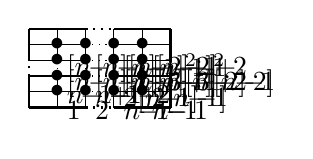
\begin{tikzpicture}[xscale=1.8]
  \draw[thick] (0,0) -- (0.4,0);
  \draw[thick,style=dotted] (0.4,0) -- (0.6,0);
  \draw[thick] (0.6,0) -- (1.0,0);

  \draw[thick] (0,1.0) -- (0.4,1.0);
  \draw[thick,style=dotted] (0.4,1.0) -- (0.6,1.0);
  \draw[thick] (0.6,1.0) -- (1.0,1.0);

  \draw[thick] (0,0) -- (0,0.4);
  \draw[thick,style=dotted] (0,0.4) -- (0,0.6);
  \draw[thick] (0,0.6) -- (0,1.0);

  \draw[thick] (1.0,0) -- (1.0,0.4);
  \draw[thick,style=dotted] (1.0,0.4) -- (1.0,0.6);
  \draw[thick] (1.0,0.6) -- (1.0,1.0);

  \foreach \x in {0.2,0.4,0.6,0.8}
  {
    \draw (\x,0) -- (\x,0.4);
    \draw[style=dotted] (\x,0.4) -- (\x,0.6);
    \draw (\x,0.6) -- (\x,1.0);
  }
  \foreach \y in {0.2,0.4,0.6,0.8}
  {
    \draw (0,\y) -- (0.4,\y);
    \draw[style=dotted] (0.4,\y) -- (0.6,\y);
    \draw (0.6,\y) -- (1.0,\y);
  }
  \foreach \x in {0.2,0.4,0.6,0.8}
  {
    \foreach \y in {0.2,0.4,0.6,0.8}
    {
      \draw (\x,\y) node {$\bullet$};
    }
  }
\draw (.2,.2) node[anchor=north west] {$1$};
\draw (.4,.2) node[anchor=north west] {$2$};
\draw (.6,.2) node[anchor=north west] {$n\!\!-\!\!1\!\!-1$};
\draw (.8,.2) node[anchor=north west] {$n\!\!-\!\!1\!\!$};

\draw (.2,.4) node[anchor=north west] {$n\!\!-\!\!1\!\!+\!\!1$};
\draw (.4,.4) node[anchor=north west] {$n\!\!-\!\!1\!\!+\!\!2$};
\draw (.6,.4) node[anchor=north west] {$2[n\!\!-\!\!1]\!\!-\!\!1$};
\draw (.8,.4) node[anchor=north west] {$2[n\!\!-\!\!1]$};

\draw (.2,.6) node[anchor=north west] {$[n\!\!-\!\!1][n\!\!-\!\!3]\!\!+\!\!1$};
\draw (.4,.6) node[anchor=north west] {$[n\!\!-\!\!1][n\!\!-\!\!3]\!\!+\!\!2$};
\draw (.6,.6) node[anchor=north west] {$[n\!\!-\!\!1][n\!\!-\!\!2]\!\!-\!\!1$};
\draw (.8,.6) node[anchor=north west] {$[n\!\!-\!\!1][n\!\!-\!\!2]$};

\draw (.2,.8) node[anchor=north west] {$[n\!\!-\!\!1][n\!\!-\!\!2]\!\!+\!\!1$};
\draw (.4,.8) node[anchor=north west] {$[n\!\!-\!\!1][n\!\!-\!\!2]\!\!+\!\!2$};
\draw (.6,.8) node[anchor=north west] {$[n\!\!-\!\!1]^2\!\!-\!\!1$};
\draw (.8,.8) node[anchor=north west] {$[n\!\!-\!\!1]^2$};
\end{tikzpicture}
}

\begin{Definition}{5-point-stencil}
  The \define{5-point stencil} consists of the sum of a 3-point
  stencil in $x$- and a 3-point stencil in $y$-direction. Its
  graphical representation is
  \begin{center}
    \includegraphics[width=.25\textwidth]{fig/5-point-stencil.tikz}
  \end{center}
  For a generic row of the linear system, where the associated point is not
  neighboring the boundary, this leads to
  \begin{gather}
    \label{eq:5-point-stencil:1}
    \frac1{h^2}\bigl[4y_k - y_{k-1} - y_{k+1} - y_{k-(n-1)} -
    y_{k+(n-1)}\bigr] = f_k
  \end{gather}
  If the point $k$ is next to the boundary, the corresponding entry
  from the matrix must be omitted.
\end{Definition}

%%% Local Variables:
%%% mode: latex
%%% TeX-master: "../notes"
%%% End:


\begin{remark}
  From now on, we will call the discrete solution $u_h$ in order to
  avoid confusion with the coordinate direction $y$.
\end{remark}

\begin{Lemma}{fd-matrix}
  The matrix obtained for the Laplacian on $\Omega = [0,1]^2$ by the
  5-point stencil on a uniform Cartesian mesh of mesh spacing $h=1/n$
  with lexicographic numbering has the structure
  \begin{gather*}
    L_h =
    \begin{bmatrix}
      D & -I \\
      -I & D & -I \\
      & \ddots & \ddots & \ddots \\
      & & -I & D & -I \\
      &&& -I & D
    \end{bmatrix}
    ,\qquad
    D =
    \begin{pmatrix}
      4 & -1 \\
      -1 & 4 & -1 \\
      & \ddots & \ddots & \ddots \\
      & & -1 & 4 & -1 \\
      &&& -1 & 4
    \end{pmatrix}
  \end{gather*}
\end{Lemma}

%%% Local Variables:
%%% mode: latex
%%% TeX-master: "../notes"
%%% End:


\begin{Theorem}{5-point-m-matrix}
  The matrix generated by the 5-point stencil is an M-matrix and the
  discrete problem
  \begin{gather*}
    L_h u_h = f
  \end{gather*}
  is stable in the sense that there is a constant $c$ independent of
  the grid spacing $h$ such that
  \begin{gather*}
    \norm{L_h^{-1}} \le c.
  \end{gather*}
\end{Theorem}

\begin{proof}
  The proof of M-matrix property is identical to the proof for 2-point
  boundary value problems, which was omitted there.  The same way as
  there, the function
  \begin{gather*}
    w(x,y) = (x-a)(b-x)(y-a)(b-y)
  \end{gather*}
  can be employed to show boundedness of $\norm{L_h^{-1}}$.
\end{proof}

\begin{Lemma}{fd2-consistency}
  The 5-point stencil is consistent of second order.
\end{Lemma}

We summarize:
\begin{Theorem}{fd2-convergence}
  The finite difference methods constructed so far for the Poisson
  equation is convergent of second order.
\end{Theorem}

%%% Local Variables:
%%% mode: latex
%%% TeX-master: "../notes"
%%% End:


\begin{proof}
  We apply the analysis of Lemma~\ref{Lemma:fd-consistency} in $x$-
  and $y$-directions separately, obtaining
  \begin{align*}
    \abs{\frac{\partial^2}{\partial x^2} u(x,y)
      - \frac{u(x+h,y) -2u(x,y) + u(x-h,y)}{h^2}} & \le c h^2 \\
    \abs{\frac{\partial^2}{\partial y^2} u(x,y)
      - \frac{u(x,y+h) -2u(x,y) + u(x,y-h)}{h^2}} & \le c h^2,
  \end{align*}
  an conclude consistency of the sum.
\end{proof}

\begin{Theorem}{fd2-maximum}
  Let $y$ be the solution to the finite difference method for the
  Laplace equation with the 5-point stencil. Then, the maximum
  principle holds for $y$, namely, if there is a point $(\mathbf x_k)$
  such that $y_k\ge y_j$ for all $j\neq k$ and $y_k\le y_B$ for any
  boundary value, then $y$ is constant.
  
\end{Theorem}
%%% Local Variables: 
%%% mode: latex
%%% TeX-master: "../notes"
%%% End: 


\begin{proof}
  From equation~\eqref{eq:5-point-stencil:1}, it is clear that a
  discrete mean value property holds, that is, $y_k$ is the mean value
  of its four neighbors. Therefore, if $y_k \ge y_j$, for all
  neighboring indices $j$ of $k$, we have $y_j = y_k$. We conclude by
  following a path through the grid points.
\end{proof}

\subsection{Fundamental solution}

\begin{Definition}
  The function
  \begin{gather}
    \label{eq:fd:fundamental}
    \Phi(x) =
    \begin{cases}
      -\tfrac{1}{2\pi} \log \abs{x} & d=2\\
      \tfrac1{d(d-2)\omega_d} \frac1{\abs{x}^{d-2}} & d\ge 3,
    \end{cases}
  \end{gather}
  for $x\in \R^d$ is the \define{fundamental solution} to the Laplace
  equation. Here, $\omega_d$ is the volume of the unit ball in $\R^d$.
\end{Definition}



%%% Local Variables:
%%% mode: latex
%%% TeX-master: "notes"
%%% End:
